\documentclass{article}
\usepackage{amsmath,enumerate,graphicx}

\begin{document}
\title{Using volumetric stereo and pattern segmentation techniques to estimate the number of jellybeans in a jar}
\author{Mark O'Meara, Alex Cope}
\date{January 30, 2104}
\maketitle

\section*{Motivation}

The challenge of estimating at a glance the number of jellybeans in a large transparent jar is a classic parlor game, one that has not flagged in appeal for many years. Even as recently as last November, prizes as large as \$125,000 have been offered at carnivals for accurate counts of immense numbers of colored beans in gigantic containers \cite{Diversion}. But far from being the sole domain of human intuition, the inherent difficulty of this problem presents several component issues that we believe are particularly conducive to computer vision techniques. And although this specific problem is relatively trivial in its scope, we suspect that the techniques devised for its successful solution could subtend many other important problems involving large count estimations, like crowd size and bird flock/fish school estimations.

   In our estimation, the "jellybean jar" problem can be decomposed into three relatively tractable subproblems: 1. 3-D modeling/measurement of the transparent container from multiple images, 2. Object segmentation of the similarly sized but multicolored jellybeans, and distinction between the partially occluded and front-layer beans, and 3. Spacefilling extrapolation and final estimation of the total jellybean count from information gleaned from these first two analyses.

   A large part of the renowned difficulty of this problem is the struggle of the human eye to correctly segment out and keep track of individual jellybeans from the horde, and this will be a steep challenge for our team as well. However, we think a few aspects of the problem lend themselves especially well to camera analysis. For one, the issue of scale, a persistent ambiguity in 3D modeling even after self-calibration and bundle adjustment, is irrelevant to this problem, as the ratio of container-to-jellybean size does not depend on any measure of absolute size. Secondly, the convexity of the containers and bright variegated colors of the jellybeans means that voxel carving could be an effective method for accurately modeling the system. And finally, the quantitative nature of this challenge, and the single integer output, will lend itself well to easy measurement of our improvement and efficacy as we progress. The ability to vary the size of the container will also allow us to limit the difficulty of the problem at first, later scaling up to much larger sizes if accurate estimations are achieved. As to the problem of segmentation, we believe that multicolored jellybeans will present a sufficient challenge, but a higher level of difficulty, viz. having all the jellybeans be of one color, is easily formulatable if desired.

\section*{Technical Approach}

\subsection*{Volumetric stereo methods}

The first component of our project will be to construct accurate 3D models of the transparent containers holding the jellybeans. Although our approach may vary as we progress, our initial plan is to employ volumetric stereo techniques to generate these models (generating accurate point correspondences needed for SRM seems prohibitively difficult considering the complex color/contour patterns of the contained jellybeans). The heterogenous colors of the jellybeans seem particularly well suited to color-based voxel carving, and we will try this method first. However, we suspect that the reflective, non-Lambertian nature of the transparent jar might confound this approach, in which case we will try the regular space carving technique shown in lecture, casting the jar against a solid backgorund. Since the jars we will test will all be convex (or at least hyperbolically concave), we do not suspect that the concavity limitations of these carving methods will be a hindrance to this approach. Once we can consistently generate reasonable 3D models of the jars, we will be ready to progress to the next step: jellybean segmentation.

\subsection*{Jellybean segmentation}

Depending on the nature of the objects in the jar, different segmentation strategies will work with varying success. For example, with multicolored jellybeans, a relatively naive color threshold algorithm would work well. Because jellybeans have a regular shape, we could then examine the shape of these segmented objects to determine level of occlusion (i.e. which objects are at the top layer), which would be used to more accurately sample the number of objects. If this naive approach is not sufficient, or we want to count objects of homogenous color, then we plan to implement the watershed algorithm, in which the grey level of a pixel is used to estimate its height and segments are drawn over local minima \cite{Watershed}, for more accurate segmentation.

\subsection*{Number estimation} 

Some experimentation will be in order to produce the most accurate results here, but we plan on estimating the total number of jellybeans using the ratio between object and space on the top layer, as well as in the first partially occluded layer, to determine the number of jellybeans that could fit in the 3D space provided. Challenges we foresee include the separation of the top and partially occluded layer; if this technique is too inaccurate (accuracy measured by manual counting) we will also try measuring via a simulation the number of jellybeans based on the ratio of jellybean to jar volume.

\section*{Progress}

Something something watershed algorithm.

\begin{figure}[h]
\centering
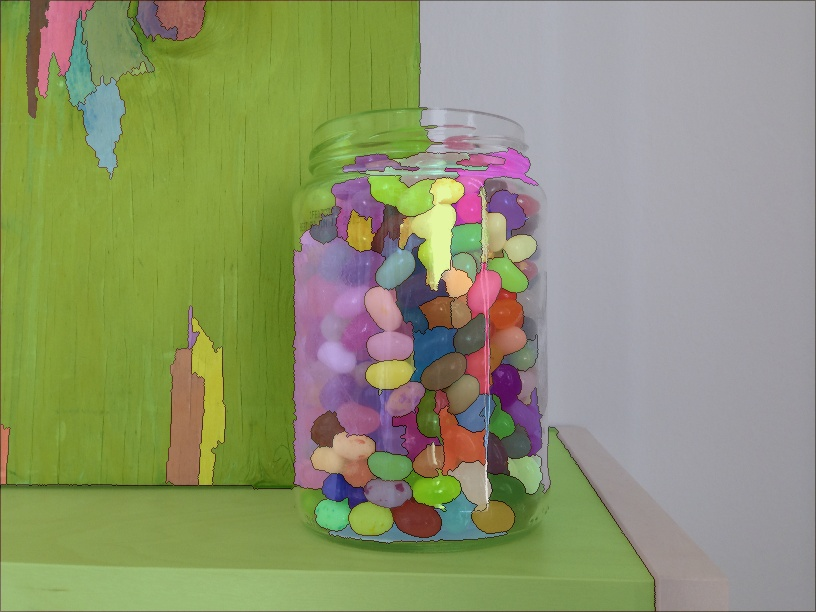
\includegraphics[width=0.8\textwidth]{../wshed.jpg}
\caption{Watershed algorithm applied to image.}
\end{figure}

\section*{Milestones}

Our problem can be neatly separated into three subproblems: 3D representation of the jar, segmentation of the objects, and geometric interpretation of jellybean number. This allows us to set clear milestones over the course of the next six weeks. Ideally, we will achieve our three subgoals in roughly two week chunks.

\textbf{By February 13,} we plan to be able to make a 3D reconstruction of a jar using space and voxel carving.

\textbf{By February 27,} we plan to be able to segment the jellybeans on the surface of the jar and estimate layering based on occlusion.

\textbf{By March 19,} we will be able to estimate based on the above data and geometric modeling the number of jellybeans in the jar. 

\begin{thebibliography}{9}

\bibitem{Diversion}
	Matheson, Whitney. (12 Nov 2013) "Silly Diversion: Can You Count the Jelly Beans?" USA Today 		[Online] Available: http://www.usatoday.com/story/popcandy/2013/11/12/jelly-beans/3506821/ [30 Jan 2014]
	
\bibitem{Watershed}
Roerdink, Jos BTM, and Arnold Meijster. ``The watershed transform: Definitions, algorithms and parallelization strategies'' \emph{Fundamenta Informaticae} 41.1 (2000): 187-228.

\end{thebibliography}

\end{document}

